\documentclass[../doc.tex]{subfiles}

\begin{document}

    \section{Création de la carte}

    \subsection{Taille et topologie de la carte}
    
    La carte est un élément crucial du jeu. En effet, toutes les mécaniques 
    (saut, échelles, course)
    deviennent inutiles si elles sont implémentées sur une carte inadéquate (avoir la 
    possibilité de grimper sur une carte plate est aussi inutile que frustrant).
    A l'inverse, une carte adaptée aux possibilités de déplacement du joueur donne à ce dernier
    l'impression de quelque chose de fini.
    \\

    Une carte spacieuse et assez verticale (accidentée et/ou avec des maisons escaladables)
    se présente donc comme la meilleure option, car elle est ainsi le moins restrictive possible.

    \subsection{Univers et design}

    Le jeu se déroule dans un univers pirate, aux Caraïbes.
    Les bâtiments doivent donc être d'inspiration hispanique,
    mais paraître peu entretenus, signe d'une longue occupation 
    pirate. La carte est une île, ce qui permet de justifier
    la limite de carte facilement (océan). En revanche, certaines 
    incohérences (skin de squelette, peut être des armes futuristes)
    permettent d'inscrire le jeu dans un registre informel, et de 
    rappeler que ce n'est qu'un jeu.
    \\

    \begin{figure}[!hbt]
        \centering
        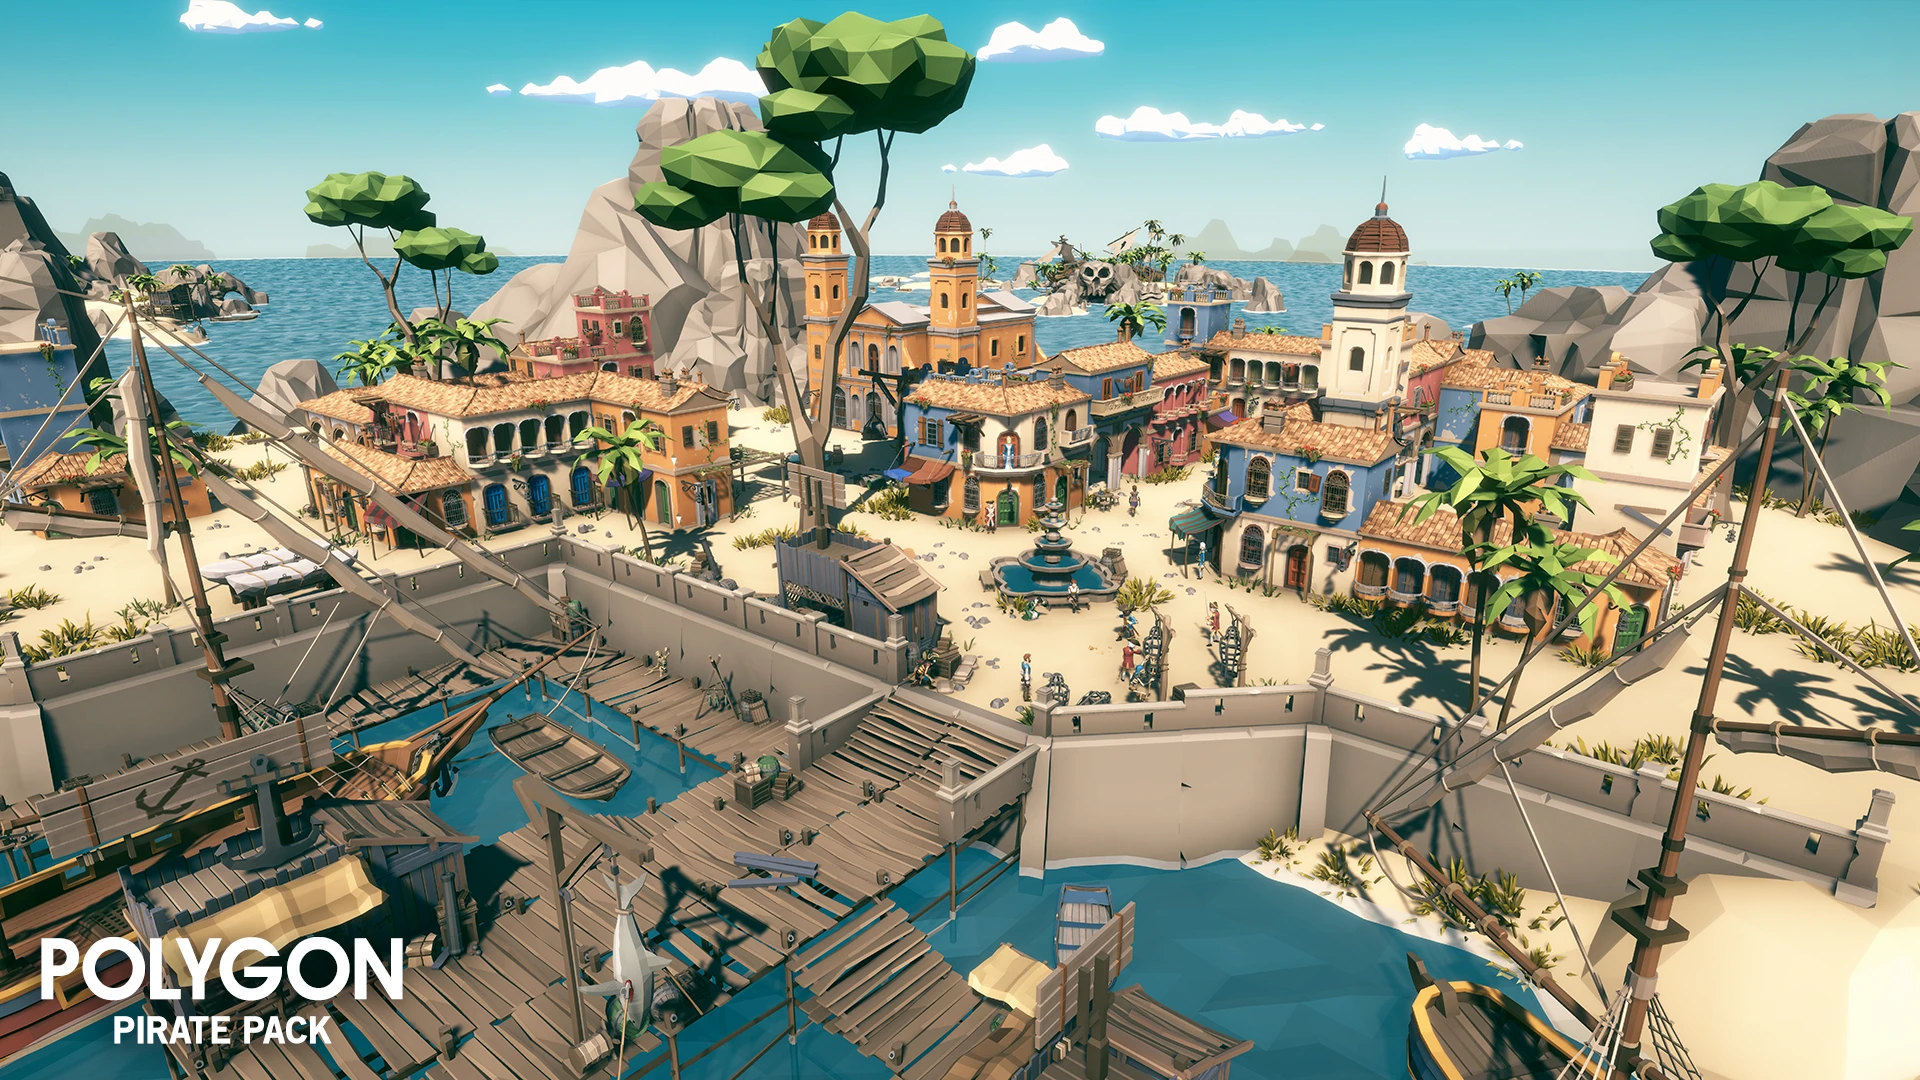
\includegraphics[scale=0.18]{polygon_pirate.png}
        \caption{Image de présentation de l'asset Polygon Pirate}
    \end{figure}


    Tous ces éléments nous ont fait opter pour l'achat d'un asset graphique chez 
    Synty Studios (POLYGON - Pirate Pack).
    Ce dernier possède de nombreux avantages, comme sa grande diversité de prefabs et 
    textures, ou encore son aspect "Low Poly", 
    c'est-à-dire en polygones, qui donne un aspect moderne au jeu tout en diminuant la 
    complexité des mesh (réduisant ainsi la 
    puissance de calcul nécessaire au jeu).
    \\ 


    


    \begin{figure}[hbt!]
        
        \begin{subfigure}[b]{1\textwidth}
            \center
            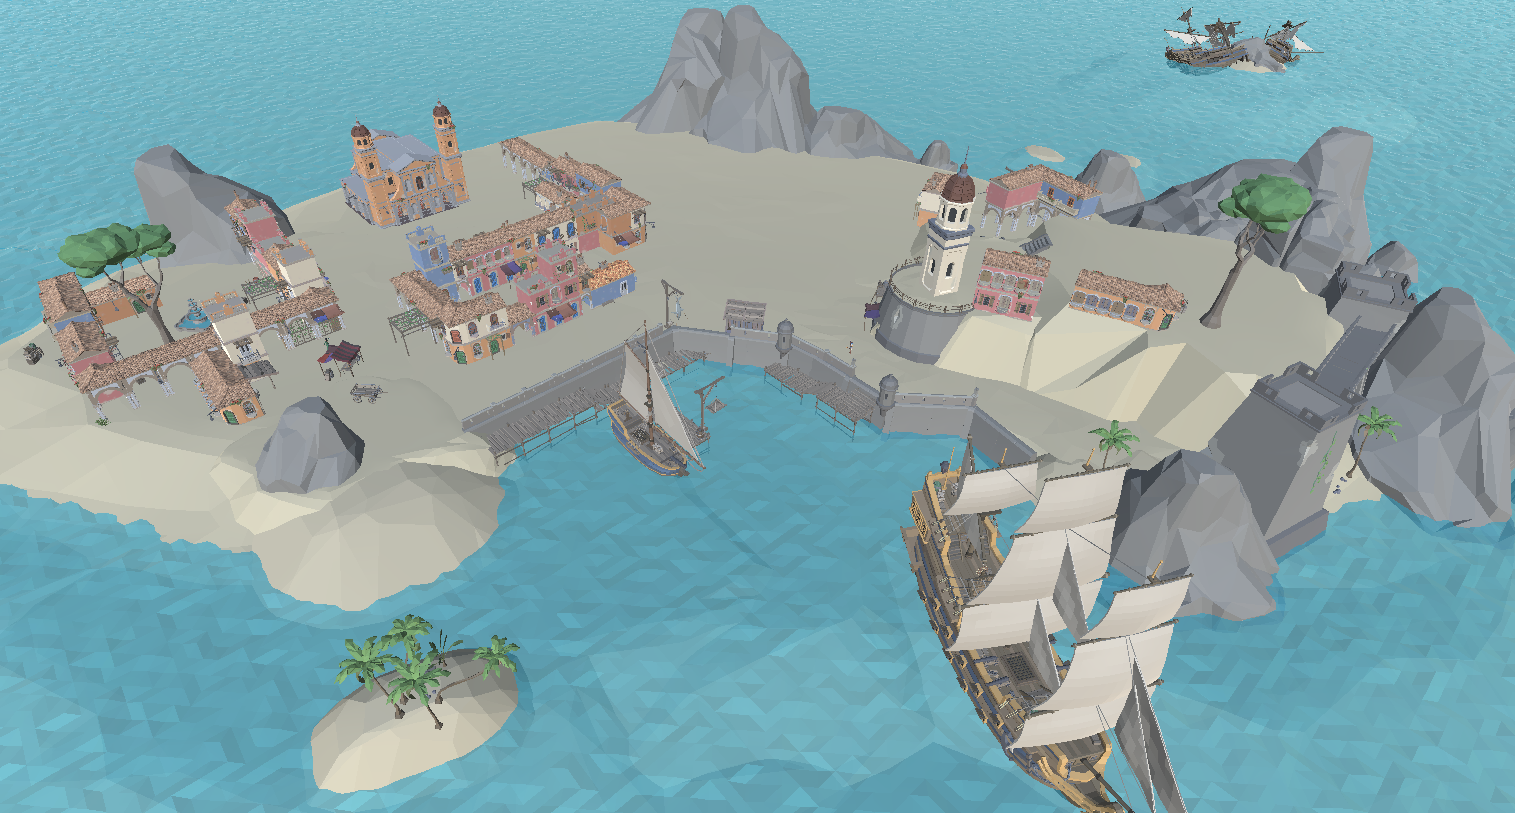
\includegraphics[scale=0.27]{map.png} 
            \caption{Vue aérienne de la carte}
        \end{subfigure}
        \vfill{}
        \begin{subfigure}[b]{1\textwidth}
            \center
            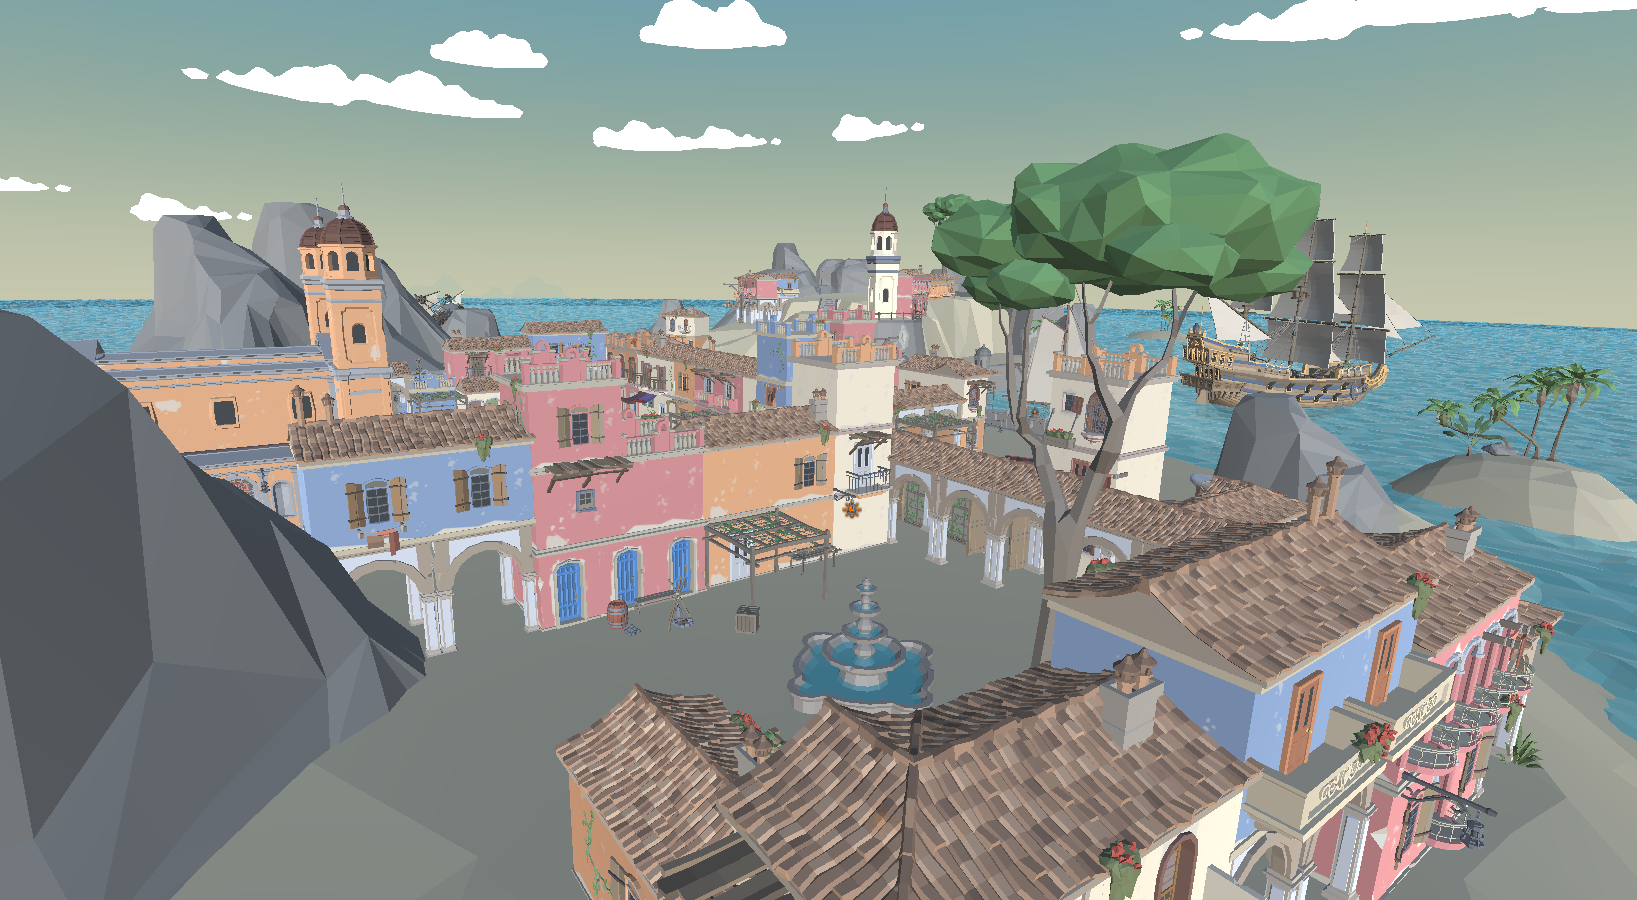
\includegraphics[scale=0.25]{streets.png} 
            \caption{Vue rapprochée de la carte}
        \end{subfigure}
        \caption{Avancement actuel de la carte}
    \end{figure}
        

    
    
\end{document}